\subsection{Test Configuration}

Our benchmark was tested on a 72-core (4 sockets with 18 cores each capable of running 2 hardware threads, totaling 144 hardware threads) Intel Xeon machine clocked at 2.50 GHz with 512 GB of RAM and 4 memory banks. The machine is running Ubuntu 14.04 with kernel verion 3.13.0-141. The with DEF code was compiled with DEF version (Whatever) and the C code was compiled with Clang 6.0, and all code was compiled with -03 level of optimisation.

During the benchmark threads were pinned programmatically to inidvidual cores initially avoiding HyperThreading and later exhausting all inidivual exection units on a single CPU with the use of HyperThreading, before migrating to another CPU socket. The scalable JEMalloc\cite{JEMalloc} allocator was used in all tests, as it had been in the Forkscan paper.\cite{Forkscan} The \texttt{numactl} Linux program was used to control which memory bank allocation was allowed to take place. The memory banks closest to the running CPUs were selected as they became active.

The microbenchmark measures the number of operations carried out over a specified amount of time rather than the time taken to exectute a specified number of iterations. The rationale for this is threads finish their iterations before other threads. The remaining threads complete their iterations with less contention in the system, skewing the overall benchmark. Our benchmark reports the number of operations per second. The primary comparison is between the leaky C and the forkscan enabled DEF implementations. Each benchmark is run for a total of 20 seconds each, with each configuration being sampled 5 times. The average of the runs is plotted with error bars show the maximum variation in each run.

\subsection{Experimental Results}

\begin{figure}[htbp!]
  \centering
  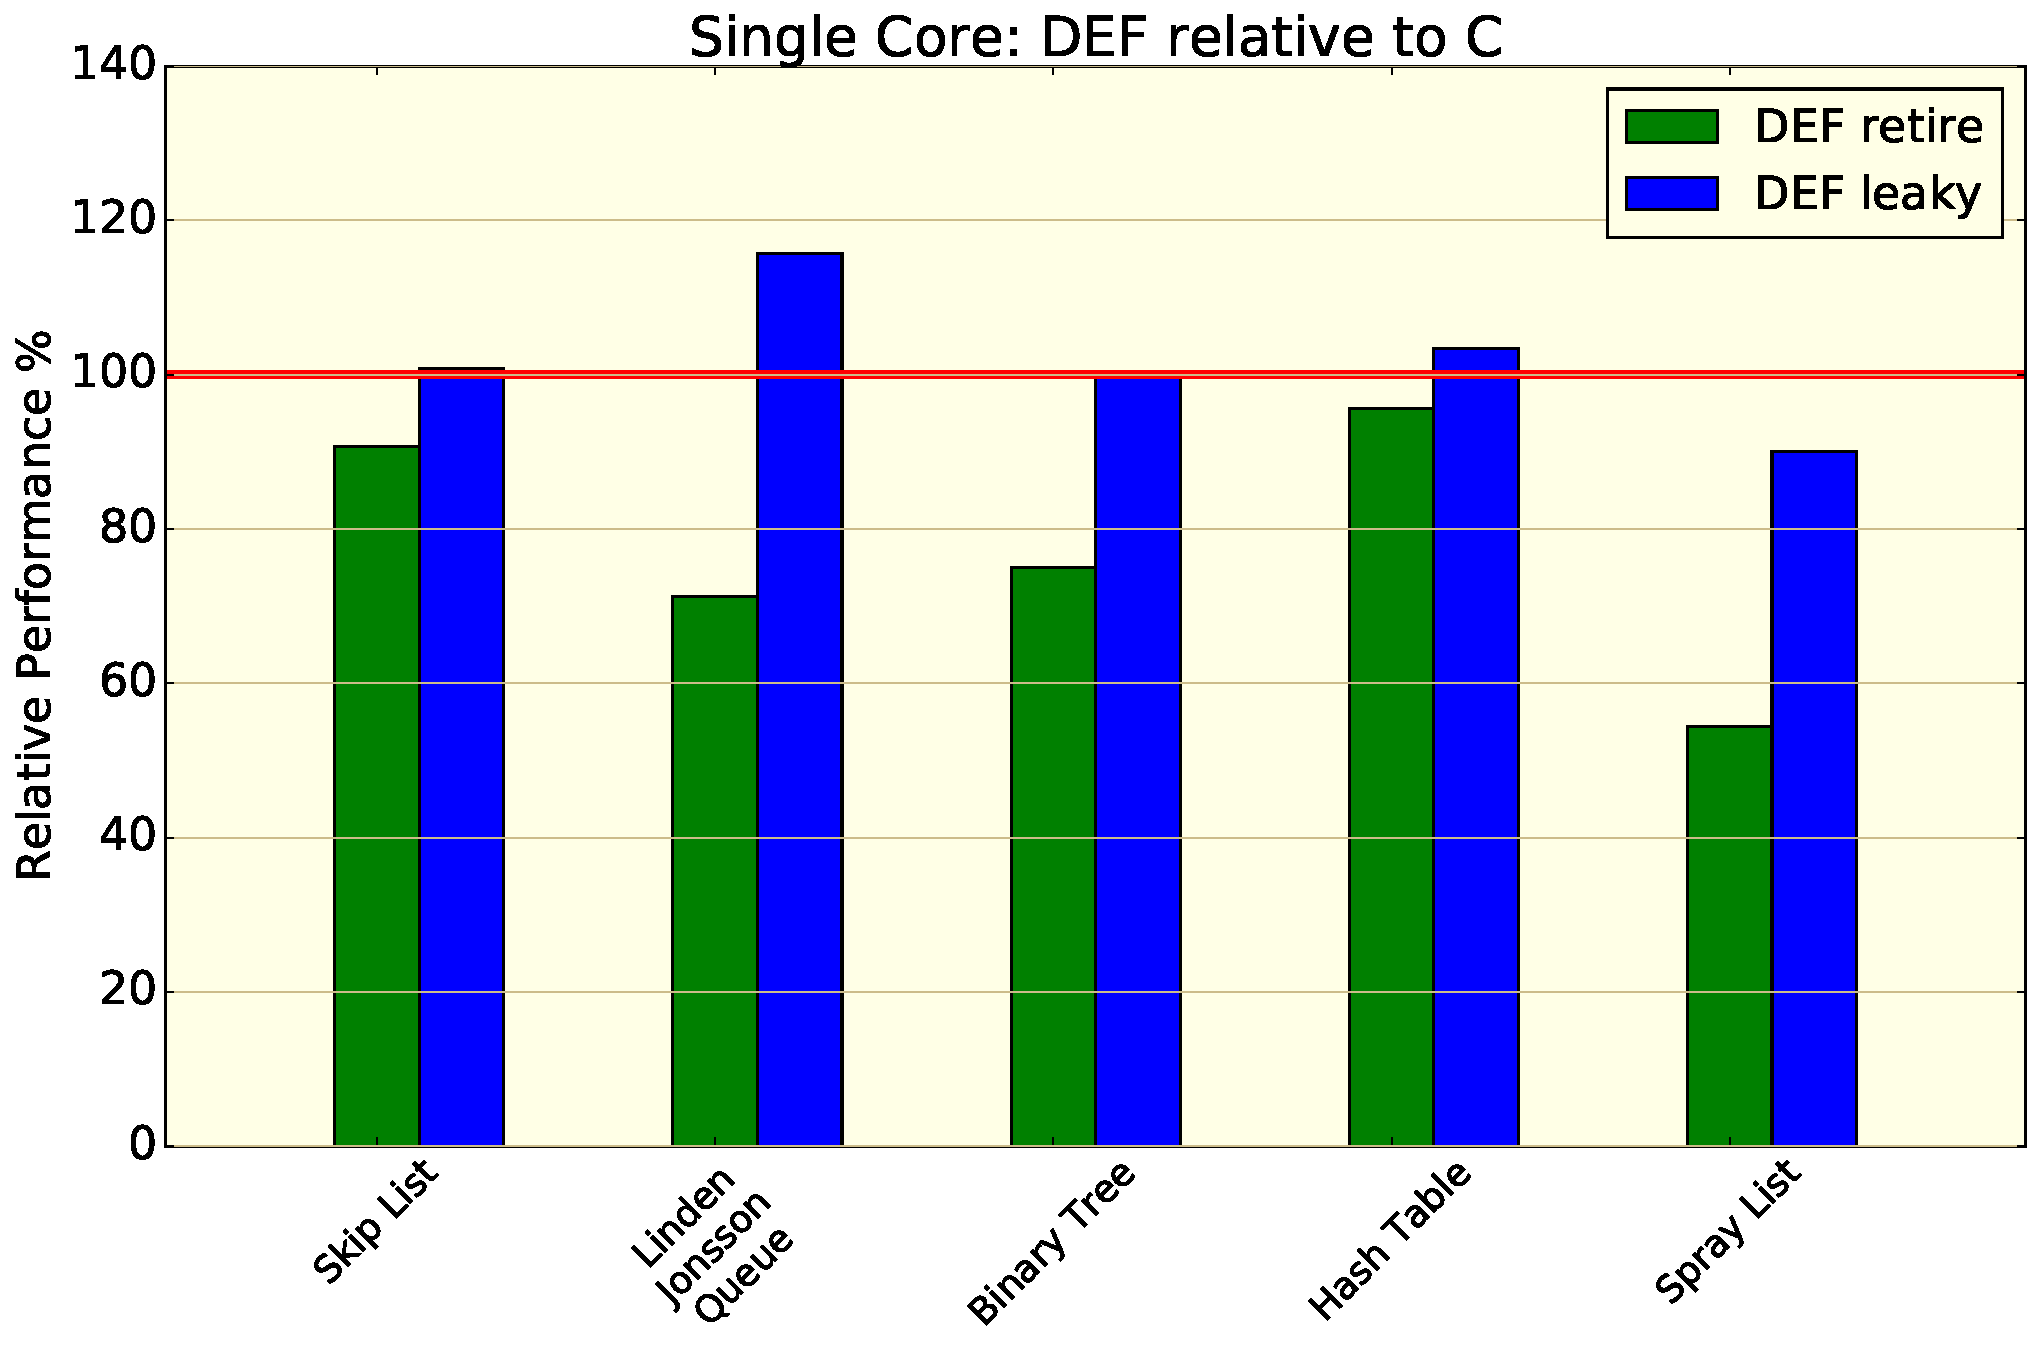
\includegraphics[scale=0.4]{gfx/RelativePerf.pdf}
  \caption{Relative performance of DEF to C on a single thread.  100\% is equivalent, and higher is better.}
  \label{fig:relativeperf}
\end{figure}

Figure \ref{fig:relativeperf} shows, for all benchmarks, single-threaded performance.  The set data structures are configured with 10\% updates, and the priority queues, naturally, are 100\% updates.  For an apples-to-apples comparison with C, a non-retiring version of the DEF code is presented.  This is a meaningful test because one expects a serial C data structure to perform better when \texttt{free} is never called than when it is, and it's no different for a concurrent data structure.  As designed, DEF is close to the machine and performs comparably in this case.

Slight degradation in performance is observed when memory is retired.  The Forkscan authors observed that reusing memory was a performance boon, but in those tests, the memory bandwidth was being saturated by the leaky code running on many threads.

\begin{figure*}[tbp]
  \centering
  \raisebox{-0.5\height}{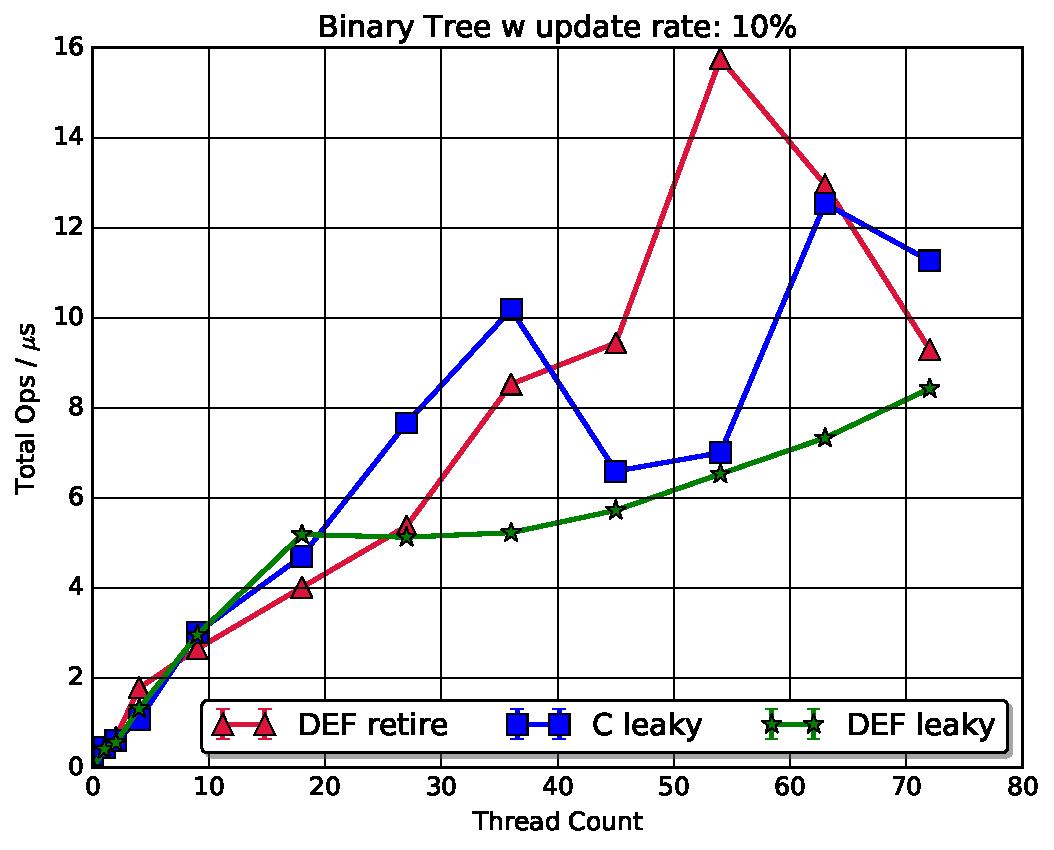
\includegraphics[scale=0.25]{gfx/BinaryTreeLight.pdf}}
  \raisebox{-0.5\height}{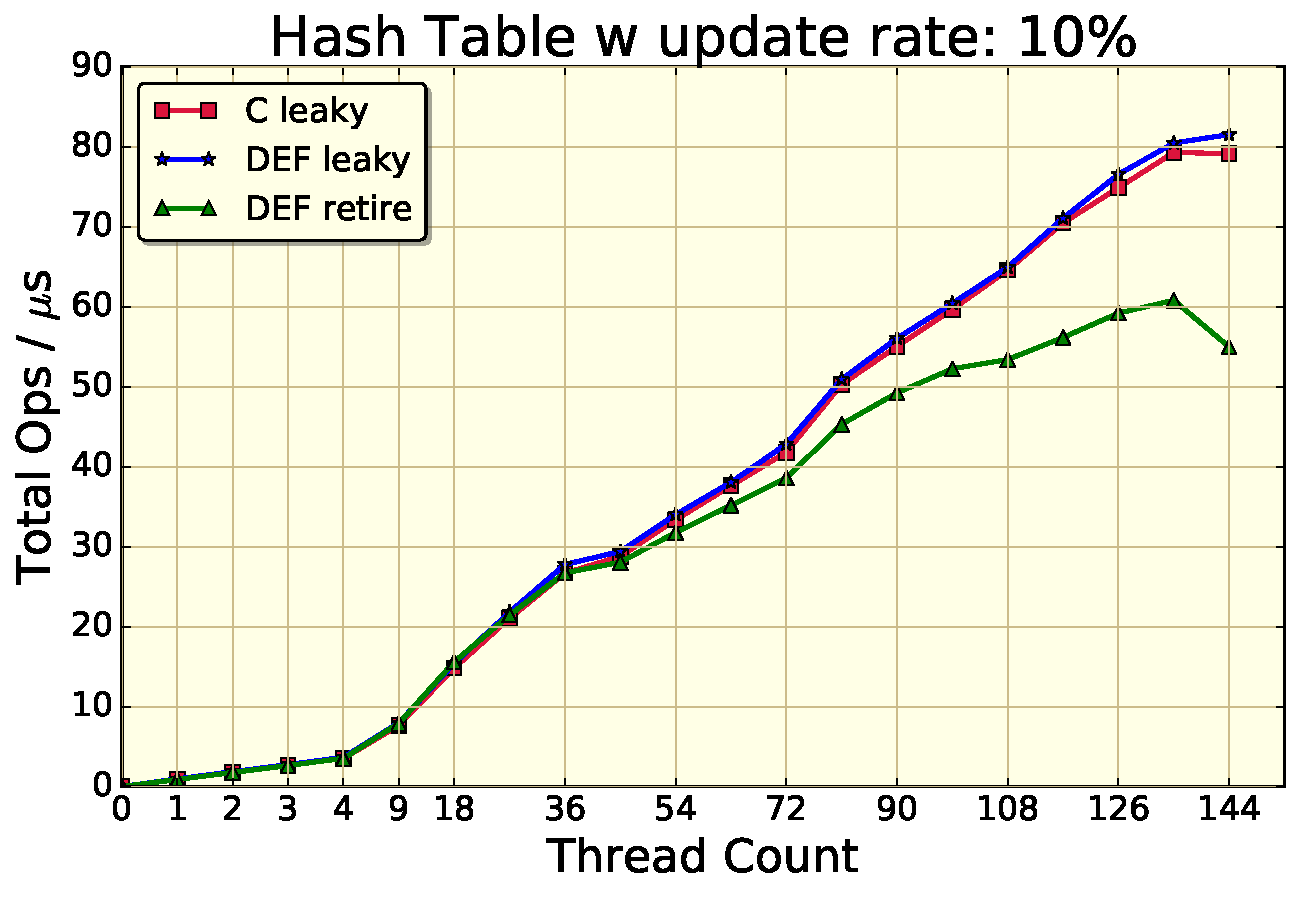
\includegraphics[scale=0.25]{gfx/HashTableLight.pdf}}
  \raisebox{-0.5\height}{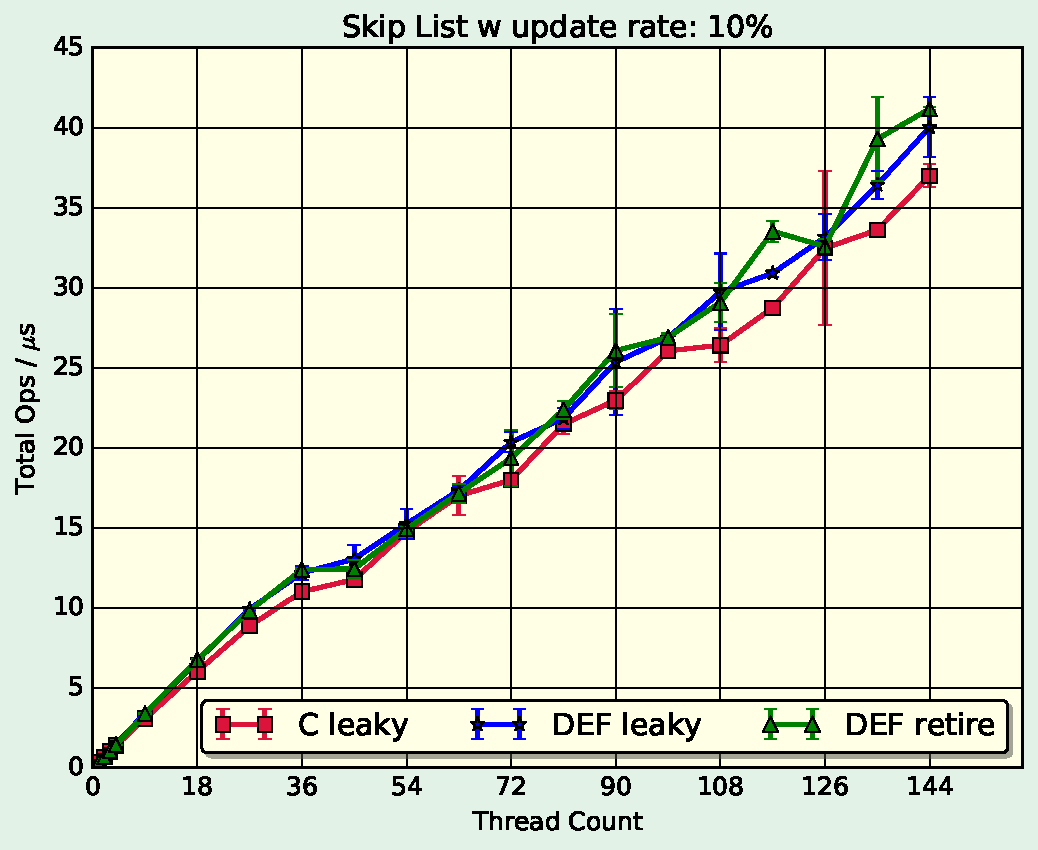
\includegraphics[scale=0.25]{gfx/SkipListLight.pdf}}
  \caption{Scalability graphs for the set data structures with 10\% updates.}
  \label{fig:workload1}
\end{figure*}

\begin{figure*}[tbp]
  \centering
  \raisebox{-0.5\height}{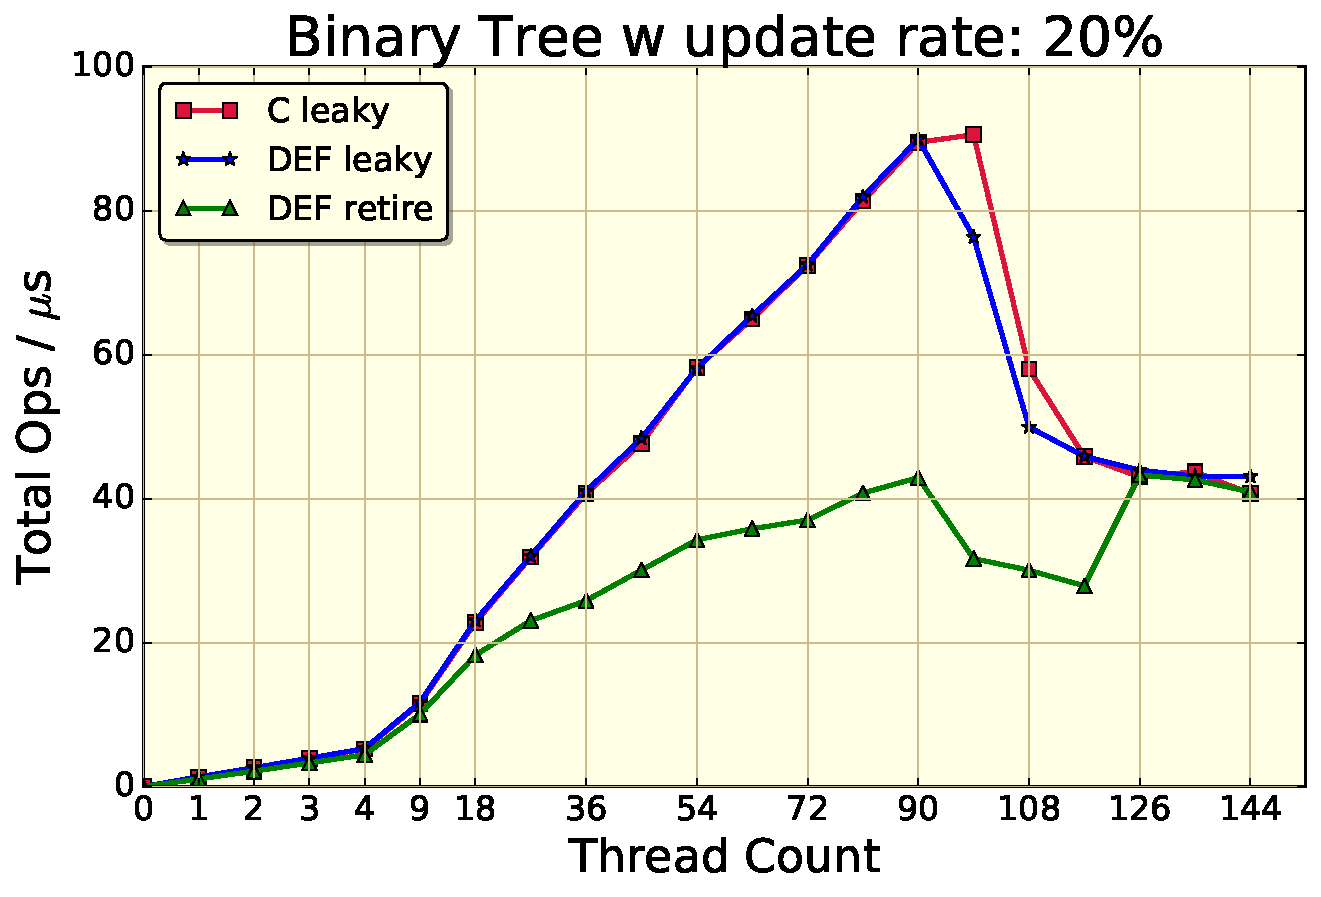
\includegraphics[scale=0.25]{gfx/BinaryTreeMedium.pdf}}
  \raisebox{-0.5\height}{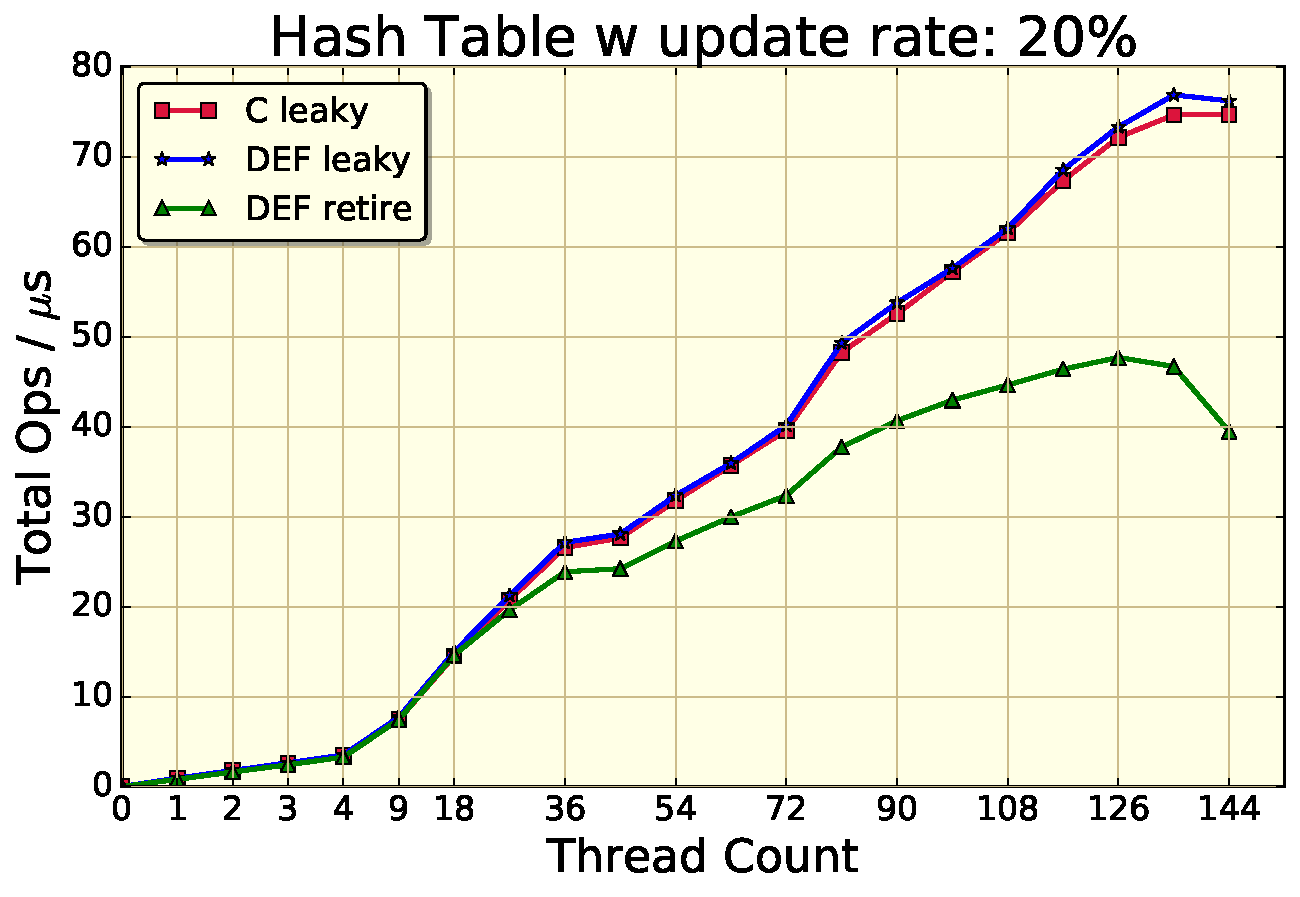
\includegraphics[scale=0.25]{gfx/HashTableMedium.pdf}}
  \raisebox{-0.5\height}{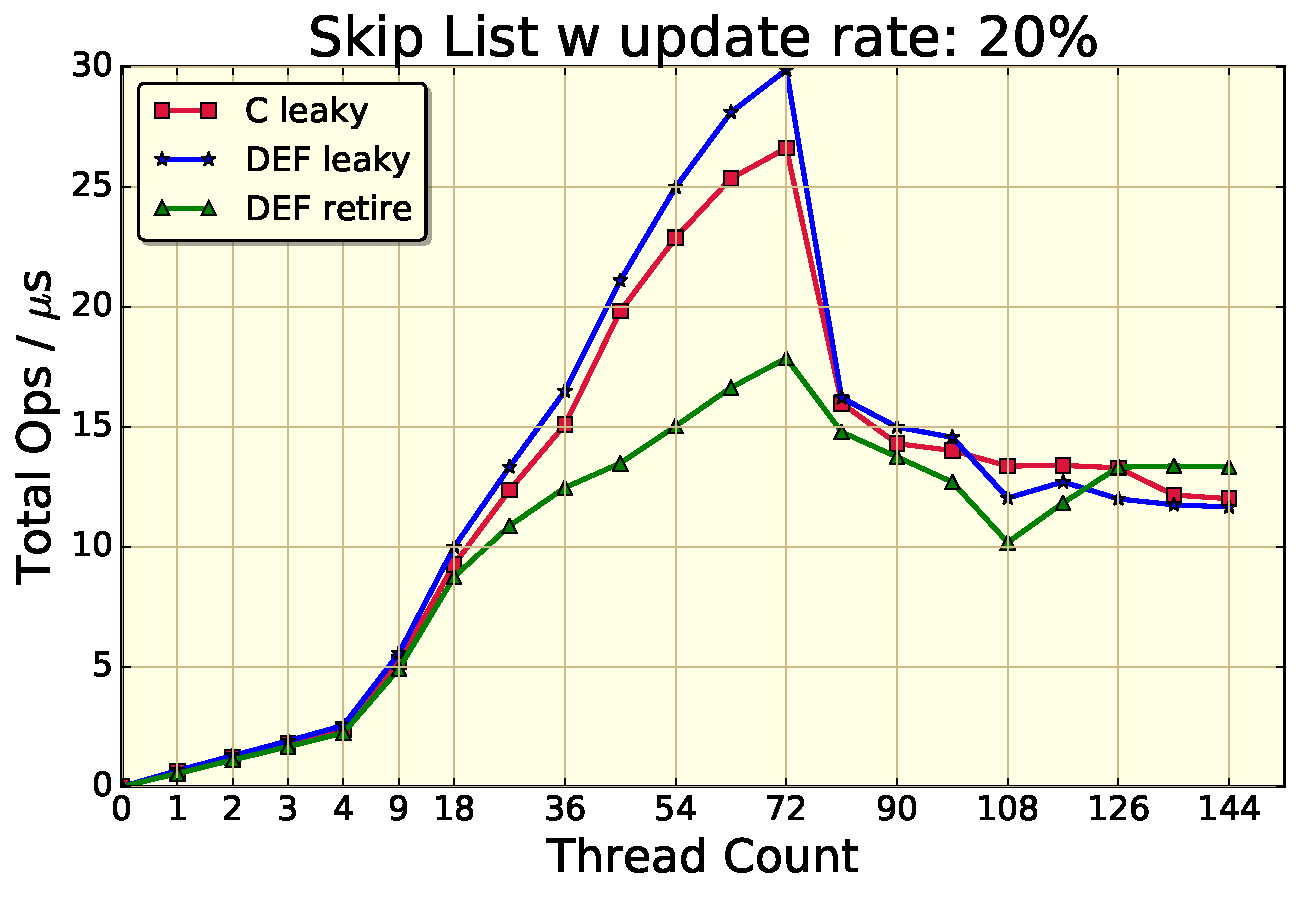
\includegraphics[scale=0.25]{gfx/SkipListMedium.pdf}}
  \caption{Scalability graphs for the set data structures with 20\% updates.}
  \label{fig:workload2}
\end{figure*}

Scalability results for the set data structures with 10\% and 20\% updates are presented in figure \ref{fig:workload1} and \ref{fig:workload2} respectively.  As above, the three configurations were tested: C, Leaky-DEF, and DEF.

\begin{figure*}[tbp]
  \centering
  \raisebox{-0.5\height}{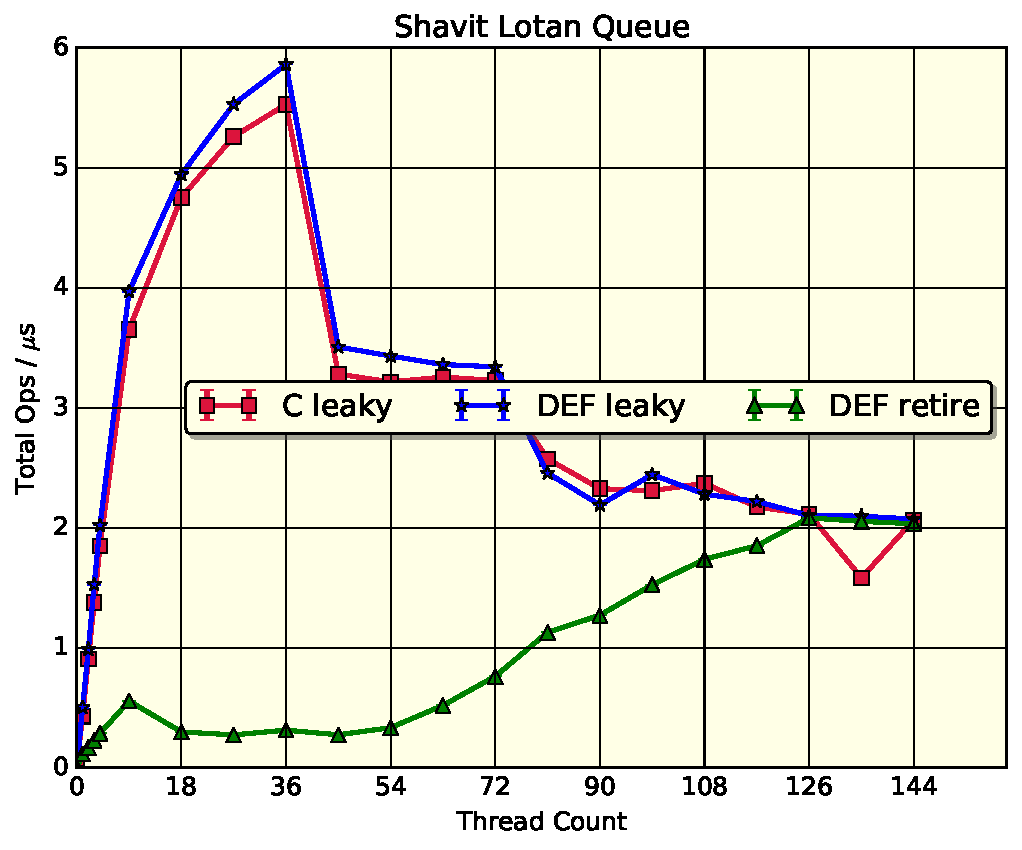
\includegraphics[scale=0.25]{gfx/ShavitLotanQueue.pdf}}
  \raisebox{-0.5\height}{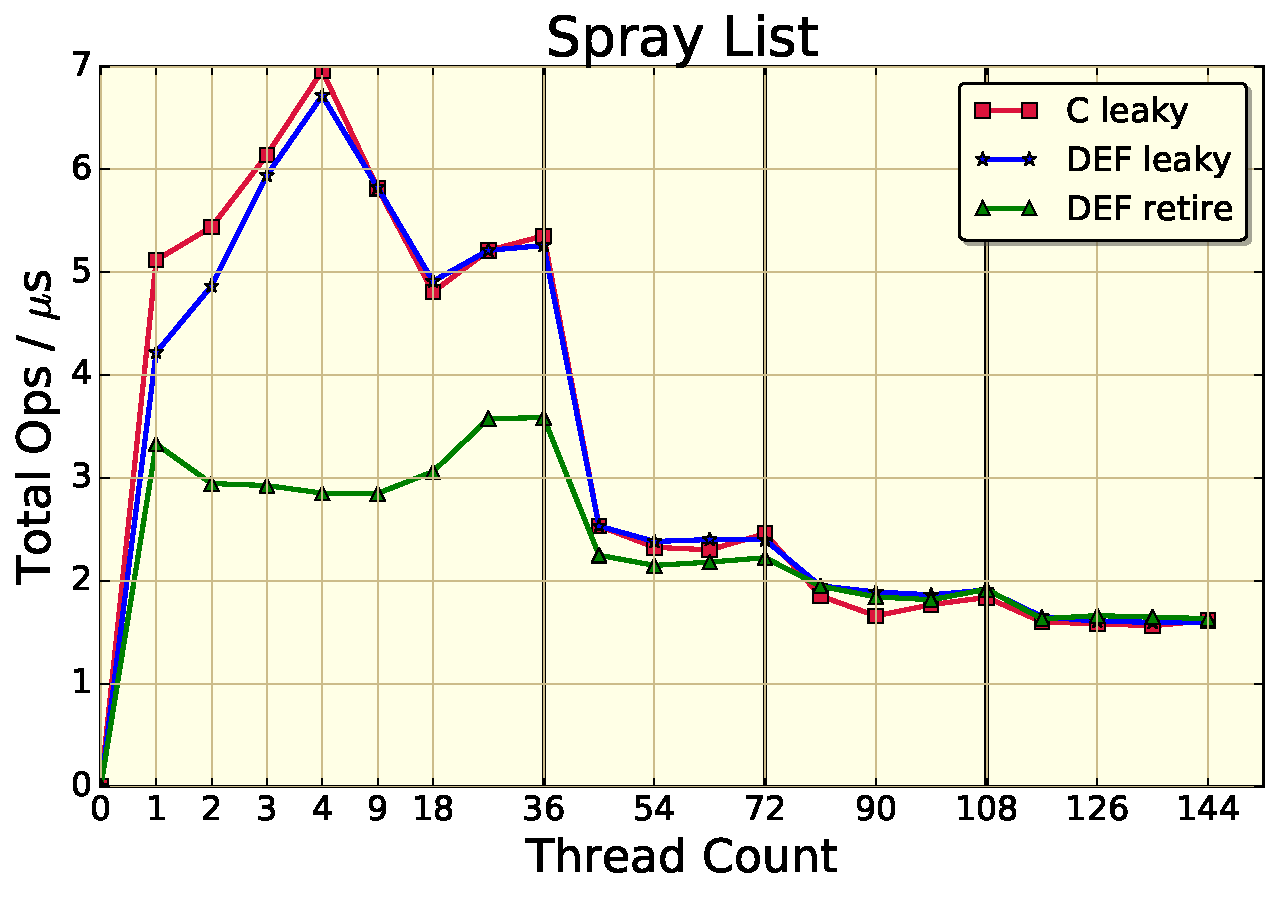
\includegraphics[scale=0.25]{gfx/SprayList.pdf}}
  \caption{Scalability graphs for the priority queues.  A priority queue's standard workload is 100\% updates.}
  \label{fig:priorityqueues}
\end{figure*}

Lastly, in figure \ref{fig:priorityqueues}, we tested the two priority queues.

